\newpage
\section*{Ziel}
Betrachung von Energieübertragung zwischen zwei miteinander kapazitiv 
gekoppelt Schwingkreise mit und ohne erzwungende äußere Anregung.
\section{Theorie}
\subsection{Gekoppelte System allgemein}
Von einem gekoppelten System spricht man, wenn zwei schwingungsfähige Systeme miteinander
Verbunden sind, sodass das eine System Einfluss auf das andere System nimmt. Dabei 
findet eine Energieübertragung von dem einen ins andere System statt.
Zudem ist das Verhalten des Gesamtsystems bei Einfluss eines äußeren periodisch einwirkenden 
Erregers intressant, da diese erzwungenden Schwingungen zu speziellen Resonanzphänomenen
führen.
\subsection{Kapazitiv gekoppete Schwingkreise}
Die zwei Schwingkreise bestehen jeweils aus einem ohmschen Widerstand, einer Induktivität $L$
(hier: Spule) und einer Kapazität $C$ (hier: Kondensator). Die Kopplung der System 
entsteht aufgrund eines Kopplungskondensator $C_k$.\\
\begin{figure}[H]
    \centering
    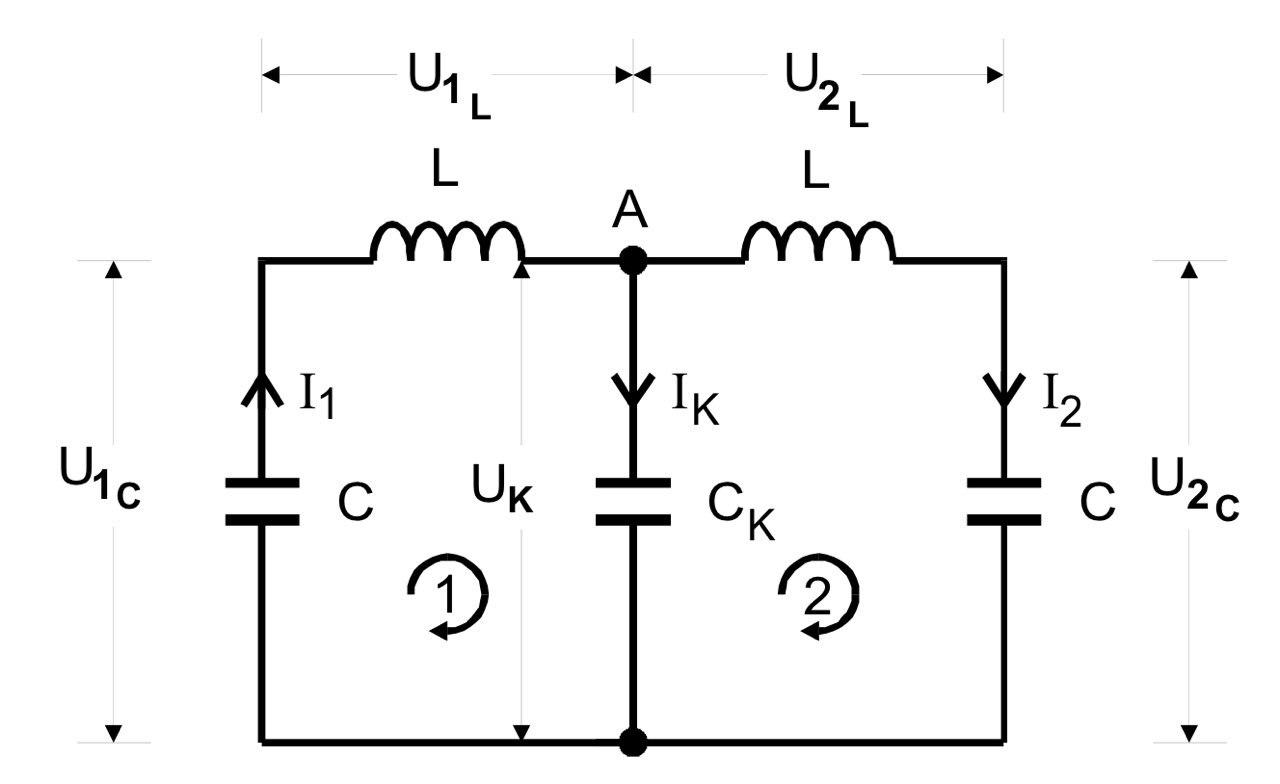
\includegraphics[width=0.5\textwidth]{bilder/schwingkreis_allgemein.jpg}
    \caption{Schaltbild von zwei Schwingkreise, die über den Kopplungskondensator $C_k$ gekoppelt sind. \cite[299]{Anleitung}}
\end{figure} 
Dabei gilt für den Strom an Punkt $A$ die Kirchhoffsche Regel
\begin{align}
    I_k&=I_1-I_2 \\
    0&=U_{1_C}+U_{1_L}+U_k\\
    0&=U_{2_C}+U_{2_L}+U_k
\end{align}
mit $U_C$ und $U_L$ ergeben sich somit zwei homogenen Differentzialgleichung zweiter Ordung, 
jeweils für den Schwingkreis 1 und 2. 
\begin{align}
    U_C&=\frac{1}{C}\int{I dt}\\
    U_L&=L \cdot \dot{I}
\end{align}
Die Lösung ergeben sich dann als:
\begin{align}
    I_1(t)&=\frac{1}{2}(I_{1_0}+I_{2_0})cos(2 \pi v^+ t)+\frac{1}{2}(I_{1_0}-I_{2_0})cos(2 \pi v^- t)\\
    I_2(t)&=\frac{1}{2}(I_{1_0}+I_{2_0})cos(2 \pi v^+ t)-\frac{1}{2}(I_{1_0}-I_{2_0})cos(2 \pi v^- t)
\end{align}
mit der Schwingfrequenz $v^+$ und $v^-$ 
\begin{align}
    v^+&=\frac{1}{2\sqrt{LC}}\\
    v^-&=\frac{1}{2 \pi \sqrt{L(\frac{1}{C}+\frac{2}{C_k})^{-1}}}
\end{align}
Dabei spricht man von den Fundermentalschwingungen, bei denen im 1 Fall $I_{1_0}=I_{2_0}$ die Anteil  aus
$(I_{1_0}-I_{2_0})$ verschwinden und somit $I_1(t)=I_2(t)$ ist, also das System phasengleich mit $v^+$ schwingt. 
Und bei dem 2 Fall $I_{1_0}=-I_{2_0}$ verschwindet $(I_{1_0}+I_{2_0})$ es 
folgt somit $I_1(t)=-I_2(t)$, also gegenphasig Schwingung mit $v^-$.\\
Lässt man ein System in Ruhe und lenkt das andere aus, also $I_{1_0}\neq 0; I_{2_0}=0$
so entsteht zwei zeitgleiche Schwingungen mit einer hohen Frequenz $\frac{\nu^+ + \nu^-}{2}$
und einer niedrigen Frequenz $\frac{\nu^+ - \nu^-}{2}$ welche man als Schwebung bezeichnet.
\begin{align}
    I_1(t)&=I_{1_0}cos(\frac{\nu^+ + \nu^-}{2}t)cos(\frac{\nu^+ - \nu^-}{2}t)\\ 
    I_2(t)&=I_{2_0}sin(\frac{\nu^+ + \nu^-}{2}t)sin(\frac{\nu^+ - \nu^-}{2}t)
\end{align}
\begin{figure}[H]
    \centering
    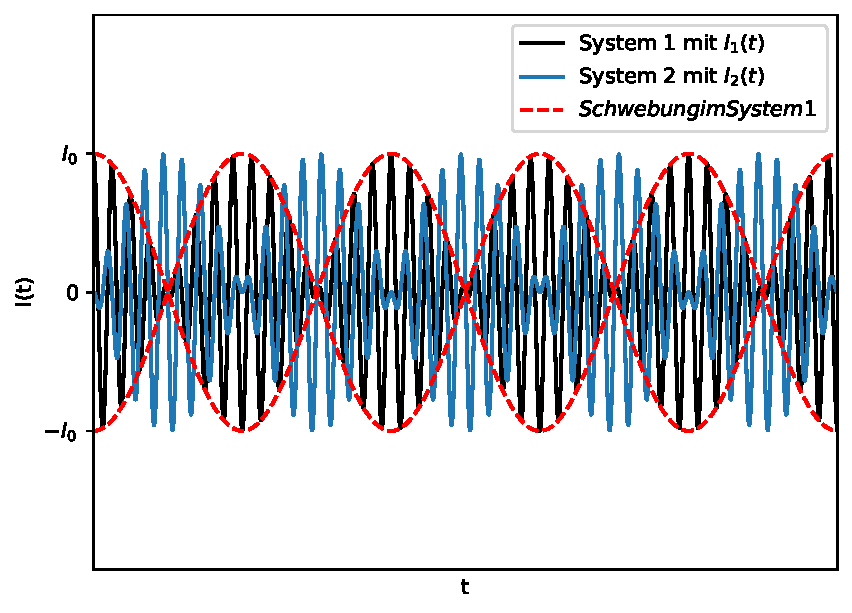
\includegraphics[width=0.6\textwidth]{build/schwebung.pdf}
    \caption{
        Darstellung einer Schwebung. Dabei wird der Energieaustausch zwischen den System deutlich.
        Das System 2 befindet sich zu Beginn in Ruhe ($I_2(0)=0$) während das System 1 zu Beginn ausgelenkt ist
        ($I_1(0)=I_0$). Energie wird dabei von System 1 auf System 2 übertragen, bis schließlich die gesamte 
        Energie in System 2 ist und der Prozess umgekehrt wiederholt wird.
    }
\end{figure}


\subsection{Gekoppelte Schwinkreise mit Erreger}
Wird ein Schwingkreis mit einer Erregerspannung (hier: eine Sinusspannung) an,
so erhält man nach den Kirchhoffschen Gesetzen
\begin{figure}[H]
    \centering
    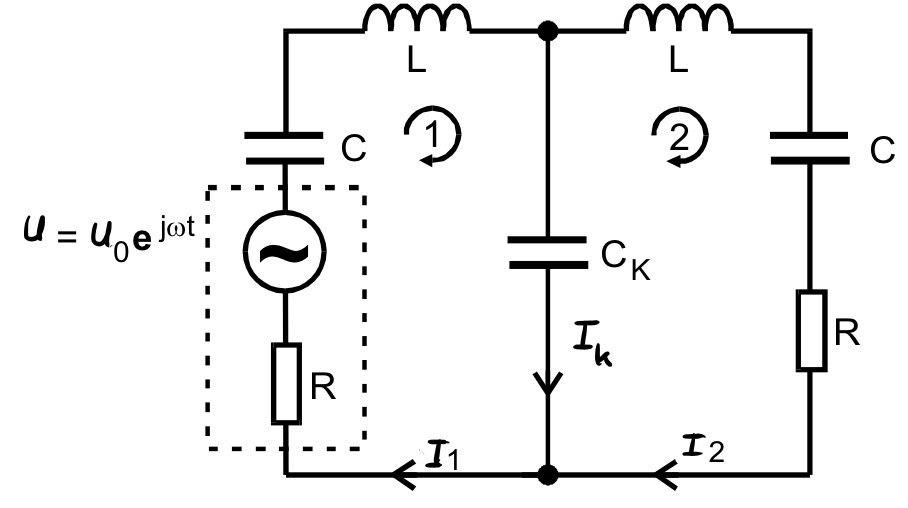
\includegraphics[width=0.5\textwidth]{bilder/schwingkreis_sinus.jpg}
    \caption{Gekoppelte Schwinkreise mit Sinusgenerator \cite[303]{Anleitung}}
\end{figure} 
\begin{align}
    U&=(z_C+z_L+z_{C_k}+z_R)I_1-z_{C_k}I_2 \label{schw1}\\
    0&=(z_C+z_L+z_{C_k}+z_R)I_2-z_{C_k}I_1 \label{schw2}
\end{align}
mit den passenden Impedanzen $z_C$, $z_L$ und $z_R$
\begin{align*}
    z_C=\frac{1}{i\omega C}&
    &z_L=i \omega L&
    &z_R=R
\end{align*}
folgt schließlich die frequenzabhängige Gesamtimpedanz $Z(\omega)$.
\begin{equation}
    Z(w)=\omega L -\frac{1}{w(\frac{1}{C}+\frac{1}{C_k})^{-1}}
\end{equation}
Daraus folgen die Maxima für den Strom $I_2(w)$ mit
\begin{align}
    |I_2(w^+)|=\frac{1}{R\sqrt{4+\frac{R^2C_k^2}{LC}}}&&
    |I_2(w^-)|=\frac{1}{R\sqrt{4+\frac{R^2C_k^2}{LC}(1+\frac{C}{C_k})}}
\end{align}

\label{sec:theorie}